\documentclass{article}
\usepackage[utf8]{inputenc}
% \usepackage[spanish]{babel}
\usepackage[english]{babel}
\usepackage{booktabs}
\usepackage{tabularx}
\usepackage{graphicx}
\usepackage{float}




\usepackage{hyperref}
\restylefloat{table}

\title{Using Random Fourier Features with Random Forest}
\author{Albert Ribes}

\begin{document}
\maketitle
\tableofcontents
\newpage

\section{Context}
    \subsection{General Framework}

    Machine Learning uses statistical models to make predictions or decisions
    when there is no known formula of feasible procedure to find the correct
    answer. In the supervised learning sub-field, it uses a collection of
    data instances and their corresponding answer to predict
    the correct outcome for new unseen data. This is known as learning.

    The theory behind this process has been developed for many time and is quite
    old. But it has not been possible to use it in real world problems until the
    recent years, when the computational power of the machines has grown so much
    that it is able to perform most of the calculations needed to ``learn'' with
    a decent level of accuracy.

    Moreover, nowadays it is relatively easy to find or produce huge datasets
    about almost any field, and that makes it possible for many businesses to learn
    from this data and to make better decisions.

    Nevertheless, the current level of learning is not enough. The error rate is still too high for some applications, and it is needed a lot of
    computation time to train a model. There is still much work to do in
    this field.
    % \begin{itemize}
    %     \item El Machine Learning es útil cuando no hay una fórmula o
    %     procedimiento factible conocido para calcular la respuesta correcta a un
    %     problema, pero sí conocemos la respuesta a varias instancias del
    %     problema, o tenemos un eurístico de cuando una respuesta es buena o mala
    %     \item La teoría detrás del machine learning hace años que está trabajada,
    %     pero ha sido necesario que la tecnología permitiera hacer esos cómputos
    %     para que se pudiera aprovechar
    %     \item Actualmente se necesitan muchísimos datos y muchísimas horas de
    %     cálculo para resolver problemas interesantes del machine learning
    % \end{itemize}
    \subsection{Into the specifics}
    The error made by an algorithm may be caused by inherent limitations of the
    data (such as random noise, lack of information, mistakes in data
    collection, etc.) or by limitations in the mathematical model behind the
    algorithm, such as having a lot of bias or variance. One way to reduce this
    last problem in to use some kind of ensemble of predictors.

    Bagging\cite{breiman94} is an ensemble technique which has shown very good results for
    some algorithms. It is known to substantially reduce the variance of a model when each of the estimators has very little correlation with the others. It
    achieves that by using bootstrap (a random sampling with
    replacement), but for most of the models this is not enough. This is why it is rarely used for any model but the Decision Tree. The instability in this
    algorithm helps each of the estimators to have low correlation.

    There exists a mapping to transform data from a given space to a different one which is called Random Fourier Features\cite{rahimi07}. It can approximate any
    shift-invariant kernel function with a randomized mapping, and has successfully
    been used to decrease the error rate of a Neural Network\cite{zhangs17}.

    In this project I try to use this mapping to increase the accuracy that can
    be achieved by models using the bagging ensemble. It is expected that it will
    enable other models than Decision Tree to produce uncorrelated estimators and
    thus reduce the variance of the model.
    % \begin{itemize}
    %     \item El error obtenido puede ser del irreducible o reducible, y éste
    %     último se debe al bias o a la varianza
    %     \item Los ensemble se usan para intentar reducir este error reducible
    %     \item Bagging necesita que los estimadores estén poco relacionados entre
    %     ellos, para reducir la variaza sin incrementar demasiado el sesgo
    %     \item Esta decorrelación la consigue en general usando bootstrap
    %     \item Pero en general solo se usa con DecisionTree porque es muy
    %     inestable, y ayuda a que esté todavía más decorrelacionado
    %     \item Los RFF son un mapeo de los datos a un subespacio aleatorio que
    %     aproxima el subespacio que mapea un shift invarian kernel
    %     \item Utilizar RFF con bagging puede ayudar a decorrelacionar más los
    %     estimadores y quizá mejorar el accuracy
    % \end{itemize}
    \subsection{State of the Art}

    It is hard to define the state of the art in Machine Learning since it still
    does not exist a certain algorithm able to solve any kind of problem.
    Nevertheless, there are some general methods used to achieve the highest
    scores.

    Deep Learning has proven to give very good results when you feed the network
    with huge amounts of data. It has been used to master some difficult games\cite{alphago16}
    and for image processing\cite{jiwan14}, among others.


    Support Vector Machines are also showing very good results using the
    kernel trick\cite{rahimi07}.
    % Support Vector Machine are also very used with the kernel trick ......

    But what is really carrying Machine Learning to another level is the possibility
    of building computation mega-clusters to train models in a way that some time
    ago would have required many years of training.

    Nevertheless, we are still not proud of the levels of accuracy we can achieve,
    and a lot of research is being done trying to increase it.

    % \begin{itemize}
    %     \item Todavía no hay un algoritmo que sea capaz de resolver todos los
    %     problemas del machine learning
    %     \item Cada proyecto tiene sus propios constraints
    %     \item Están empezando a ser factibles métodos con macro-computaciones,
    %     como el deep learning, y está dando buenos resultados
    %     \item Ahora mismo uno de los factores limitantes es la potencia de
    %     cálculo
    %     \item Todavía no estamos contentos del todo con el accuracy que obtenemos
    %     de nuestros algoritmos
    %     \item Métodos como nystroem para aproximar kernels están consiguiendo
    %     muchísima atención
    %     \item Deep Learning
    % \end{itemize}
    \subsection{Problem to solve}
    The problem is always the same: we want to achieve higher accuracy while
    solving our problems. The proposed solutions to try to solve this problem
    are:

    \begin{itemize}
        \item \textbf{Increase the computation time}: either by using very
        powerful supercomputers or by using more time.
        \item \textbf{Use better datasets}: the larger and complete a dataset
        is, the better the accuracy will be.
        \item \textbf{Improve current algorithms or create new ones}: by making
        scientific studies
    \end{itemize}

    In this project I try to increase the accuracy with the third method. It has
    the advantage of being the cheaper in the long term and more affordable.

    % El problema sigue siendo el accuracy. Todavía no se obtiene todo el que
    % sería deseable
    %
    % Nos vamos a centrar en los problemas de clasificación
    % \subsection{Solutions to the problem}
    % \begin{itemize}
    %     \item Más tiempo de cómputo
    %     \item Computación en paralelo
    %     \item Mejores algoritmos
    %     \item Datasets más grandes
    % \end{itemize}
    % \subsection{Solution Proposed in this project}
    % Se propone la solución de mejorar los algoritmos, viendo si podemos recucir
    % el error de algunos existentes
    %
    % Tiene la ventaja de que es genérica para cualquier tipo de problemas. Es decir,
    % en algunas circunstancias no te puedes permitir pedir un dataset más grande.
    % Pero lo que propongo sí que podrías hacerlo con los mismo datos.
    %
    % También se espera que no incremente demasiado la cantidad de cómputo que se
    % tiene que hacer, por lo tanto es más barato

% \section{Context}
%
% Machine Learning is a science which studies how algorithms and mathematical
% models which computer systems use can learn to give
% correct answers to many problems given some training data. When the training
% data consists on instances with some attributes and the correct answer to it,
% it is called Supervised Learning. In this sub-field, we try to solve classification and regression problems.
%
% In classification we want the algorithm to predict the correct class to which an
% instance belongs among two or more classes. For example, we may want to know if
% an email is spam or not. In regression the task is to
% precict a numerical value for the new instances. For example, we may want to predict the market price of a house.
%
% The techniques used for this problems are useful when there is no known
% formula or feasible procedure to compute the correct answer, but we do know
% the correct answer to many instances of the problem.
%
% Most of the times the information we have about the world is mistaken or
% incomplete, and so we don't want the models to adjust totally to the data, but
% to be able to ignore the noise in the data and to learn the hidden
% properties of the data. This is called generalize.
%
% When a model tries to match every single value of the data rather than
% generalize it is called over-fitting. Normally, in this cases the models achieve
% very good scores when tested with the data it has already seen, but performs
% poorly when tested with new unseen data. This is not the expected behaviour.
%
% It most of the cases the error that Machine Learning models make is a
% combination of bias and variance error.
%
% \paragraph{Bias}
% Bias is the systematic error due to erroneous assumptions in the learning
% algorithm. It can cause an algorithm to miss the relevant relations between
% features and target outputs.
%
% \paragraph{Variance}
% Variance is caused by a high sensitivity to small fluctuations in the training
% set. In can cause an algorithm to learn from the random noise in the training
% data.
%
% The objective in Machine Learning is to minimize these sources of error, but it
% is a hard job, since normally decreasing on of them will increase the other. One
% way to reduce them is to use an ensemble of estimators. Bagging is one example
% of ensemble method which tries to reduce the variance of an estimator.
%
% It is well suited for very unstable methods. This is, methods which produce
% very different models given slightly different datasets. In bagging, you train
% many instances of the same model encouraging them to have very little
% correlation, and then make all of them predict on the test data. The answer that
% has the majority of the votes is the chosen one.
%
% However, it is important for the models in the ensemble to disagree with the
% answers, just as a committee of experts needs to have different opinions to unleash
% all it power. If all of them say the same, there is no need for a committee.
%
% On the other hand, it's quite common in Machine Learning to perform a mapping
% of the original data to a different feature space, in order to ease the work
% of the models in separating the instances of the problem. Kernel functions are
% extensively used with Support Vector Machines in order to allow them to work
% for non-linear problems.
%
% There exists a special mapping called Random Fourier Features which is able to
% approximate some kernel functions to a randomized feature space. It has shown
% to be useful in Support Vector Machines by replacing the kernel function and
% reducing the amount of computation needed to do the trick, but it is not
% restricted to this usage.
%
% In this project I explore the opportunities that this mapping brings to reduce
% the error rate of some Machine Learning algorithms. I will use it together with
% bagging to try to reduce the error rate.
%
% As stated above, bagging needs its estimators to have very little correlation
% in order to be able to generalize. That is the reason why bootstrap is used to
% resample the dataset to each of the estimators, and that's also the reason
% why it is usually applied to decision trees (generating the Random Forest
% algorithm): the instability of this method makes it easier for each of the trees
% to have low correlation.
%
% Random Fourier Features allows us to generate various different random
% mappings for the same instances, thus having many approximations of the same
% points. Used together with bagging it can be used to decrease even more the
% correlation between each of the estimators, possibly increasing the accuracy.
%
% Now, this method makes it meaningful to use the bagging technique with other
% more stable methods than Decision Tree. The unstability of this model was very
% helpful to decrease the correlation of each of the trees, while it didn't make
% sense to use more stable methods with bagging, since each of the estimators
% would predict almost the same results. Now, using Random Fourier Features to
% train each of the estimators will de-correate them even if it is a stable method.


% \section{Contextualización}
%     \subsection{¿En qué contexto está enmarcado mi TFG?}
% En Machine Learning se intentan resolver problemas de clasificación o de
% regresión. Esto consiste en, dados unos datos y una respuesta a estos datos,
% ser capaz de sacar las respuestas correctas a nuevos datos (que no se han visto
% anteriormente).
% Las respuestas pueden ser poner a un elemento dentro de una clase, o predecir
% una variable numérica.
%
% Los datos que se pueden recibir también pueden sar categorías o variables
% numéricas.
%
% Normalmente ocurre que los datos que tenemos son incompletos o que tienen un
% poco de ruido aleatorio que dificulta el aprendizaje. Por eso mismo no es
% deseable que los modelos se ajusten con exactitud a los datos. Eso sería
% sobreajustar.
%
% Cuando un modelo sobreajusta, lo que ocurre es que no está generalizando, sino
% que memoriza de los datos que está viendo. Cuando se le pide al modelo predecir
% sobre datos que todavía no ha visto, obtiene muy malos resulados, porque no ha
% llegado a generalizar, sino a memorizar.
%
% Normalmente uno intenta tener la máxima precisión con los datos que ve sin
% llegar a sobreajustar sobre ellos. Eso es aprender.
%
% El error que cometen los modelos puede ser de dos tipos distintos.
%
% \subsubsection{El sesgo}
% El sesgo es el error sistemático que se comete en todas las predicciones. El
% ejemplo es el tirador de dardos que siempre le da a la posición 4, pero nunca
% da en el centro. Tiene muy buena puntería, pero no le está dando en el sitio
% correcto.
%
% \subsubsection{La varianza}
% La varianza es el error que se comete entre cada una de las predicciones.
% Puede ocurrir que las predicciones siempre queden más o menos alrededor de la
% respuesta correcta, pero que individualmente ninguna acierte. Probablemente si
% se hiciera el promedio de todas las predicciones, quedaría en la respuesta
% correcta.
%
% El ejemplo sería el tirador de dardos que tira y siempre queda más o menos
% alrededor del centro, algunas veces más a la derecha, otras más a la izquierda,
% otras más arriba, otras más abajo. El promedio de todas ellas quizá queda en
% el centro.
%
%
% Pues normalmente el error que cometen los modelos de Machine Learning es una
% combinación de estos dos errores. Algunos cometen más de un tipo que del otro.
%
%
% Existen formas de reducir el error que se comete de un tipo, normalmente a
% costa de incrementear el otro. Una de las formas es el ensembling.
%
% \subsubsection{Ensembling}
%
% Consiste en hacer un comité de modelos que predigan sobre unos datos.
%
% Nota mental: bagging reduce la varianza
%
%
% Se dice que un algoritmo o modelo es estable si con pequeñas variaciones en el
% dataset se aprendizaje los resultados que obtiene son más o menos los mismos,
% no hay mucha diferencia.
%
% Decision Tree son muy intestables, mientras que Logit es más estable.
%
% Bagging  se adapta naturalmente a Decision Tree, pues es inestable y suaviza
% el aprendizaje. No tiene mucho sentido hacer bagging con Logit, pues al ser tan
% estable los estimadores no discreparán demasiado.
%
% Sí cobra un sentido hacerlo si usamos RFF con Logit, pues entonces los
% estimadores individuales ya discrepan.
%
% Hablar del tema de la correlación entre los learners
%
%
%     \subsection{¿Cómo se gestiona actualmente el problema?}
% Con el Machine Learning el problema es que quisiéramos exigirle más de lo que
% actualmente puede hacer. Queremos más precisión y más velocidad de
% entrenamiento, y no hay un método sistemático para conseguirlo. Para algunos
% problemas habrá que dedicar más tiempo de entrenamiento, para otros serán
% necesarios datasets más grandes o mejor hechos. Algunos necesitan modelos
% de predicción más sofisticados, y algunos problemas todavía no se pueden tratar.
%
% Nosotros estamos probando lo de los modelos más sofisticados para ver si podemos
% sacar mejores predicciones o la misma precisión pero con menos tiempo de
% entrenamiento.
%
% De todos modos, la mayoría de formas de atacar el problema se pueden combinar
% entre ella, de modo que no se están comiendo el terreno. Todas colaboran para
% alcanzar el mismo fin. Simplemente, hay que centrarse en alguna de ellas para
% ver qué puede ofrecer.
%
%     \subsection{¿Existen productos similares actualmente en el mercado?}
% Lo dicho anteriormente. Para conseguir mejores resultados se suele recurrir:
% \begin{itemize}
%     \item Datasets más grandes
%     \item Más tiempo de entrenamiento
%     \item Modelos más sofisticados
% \end{itemize}
%     \subsection{Comparación en profundidad de las soluciones}
% Lo de los datasets más grandes o más tiempo de entrenamiento suele ser una
% solución que funciona, pero es bastante naive, trabajar por fuerza bruta.
% Además, no es algo que cualquiera pueda hacer. La mayoría de problemas que se
% atacan explotando alguno de estos métodos solo pueden ser atacados por grandes
% empresas que pueden invertir mucho tiempo y dinero.
%
% Por el contrario, métodos más elaborados parece ser la forma adecuada de
% proceder, aunque también es la más lenta y la que requiere más trabajo de pensar.
%
% Pero todas las formas pueden trabajar juntas para resolver los problemas.

\section{Planning}
    \subsection{Original Planning}

    In the original planning of this project the scope was
    expected to be limited to the study of Random Fourier Features with the
    Random Forest algorithm. After checking that accuracy could not be increased
    to this model, it was changed to cover also other models, such as Logistic
    Regression and Support Vector Machine with Linear Kernel.

    Furthermore, it was expected to deliver it on June 2018, and that was not
    possible.

    The expected planning was:

    % 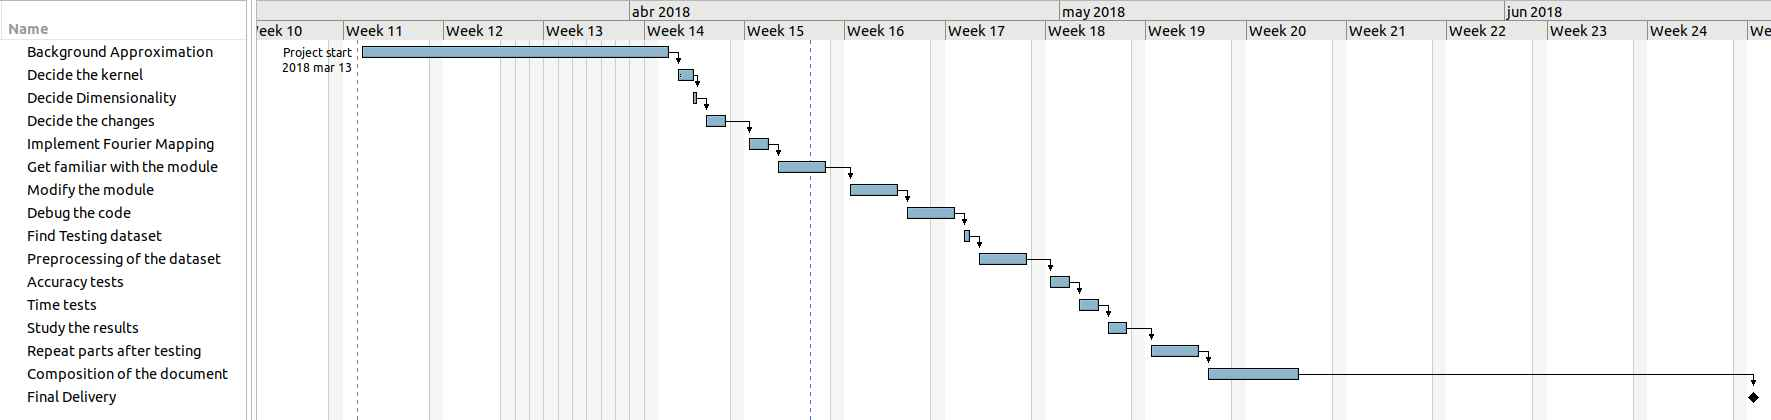
\includegraphics[width=3cm, height=4cm]{planning.jpg}
    \hspace*{-3cm}
    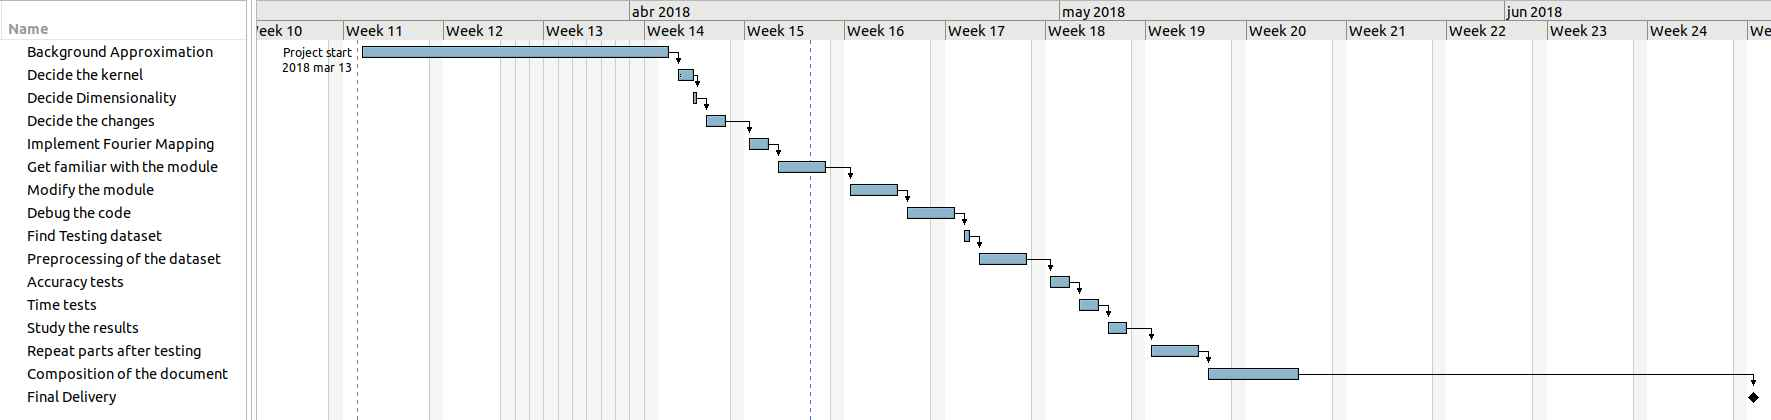
\includegraphics[width=17cm, height=7cm]{planning.jpg}


    % \begin{itemize}
    %     \item La idea inicial era trabajar solo con DecisionTree
    %     \item La fecha para la que pensaba entregar
    % \end{itemize}

    \subsection{Problems encountered with original planning}
    I encountered many problems with the original planning, both in the
    setting and in the execution. The problems were:
    \begin{itemize}
        \item \textbf{Very few knowledge of the study field}: in the beginning of the project I didn't have a clear image of how the whole project
        would be. I lacked much of the knowledge that I would need in the
        project, and was not able to write a realistic planning.
        \item \textbf{Naive assumption of success}: I expected to find good
        results on the first experiments I performed and didn't have a plan for
        when they failed.
        \item \textbf{Programming time underestimated}
        \item \textbf{Meetings with the project director}: I didn't have a good
        planning on when to meet the director of the project, and time passed
        without advancing on the work.
        \item \textbf{Communication problems}: for some time it was not possible
        to meet the director of the project physically, due to a sick leave of
        3 months. For this reason the communication was too slow.
        \item \textbf{Lack of initiative}: during the whole project I've been
        blindly following the path proposed by the director, not knowing where
        we were going. Thus, I needed constant feedback and was not able to
        advance without his advices.
        \item \textbf{Lack or rigour in following the planning}:
        the planning was not checked during the project.
    \end{itemize}
    % \begin{itemize}
    %     \item No me ceñí a lo que tenía previsto, y no llegué a tiempo
    %     \item Esperaba encontrar buenos resultados rápidamente, y no fue así
    %     \item Subestimé el tiempo que necesitaría para programar los tests
    %     \item No tenía una idea clara ni los conocimientos necesarios, y por
    %     lo tanto la planificación estaba mal hecha, no podía saber qué cosas
    %     eran importantes y qué cosas no lo eran
    %     \item El profesor estuvo enfermo
    %     \item No estuve a tiempo para entregarlo el cuatrimestre pasado
    % \end{itemize}
    \subsection{Proposed new planning}
    % TODO la fecha de entrega
    % La fecha de entrega

    As the contents of the project have changed from the original planning,
    It is needed to define a new set of tasks to finish the work. The ones which
    still need to be done are:

    % Enterarme de las fechas para las que tengo que ir entregando cosas
    % Ahora mismo, lo que me queda por hacer es:
    \begin{table}[H]
% \begin{tabular}{|l|l|}
% \begin{tabular}{|p{8cm}|p{2cm}|}
\begin{tabular}{|p{0.8\linewidth}|p{0.2\linewidth}|}
\hline
\textbf{Task} & \textbf{Time (h)} \\ \hline
% Escribir trabajo & 50\\\hline
Write the project document & 50\\\hline
% Probar de hacer un ensemble simple de DT y ver si funciona & 5\\ \hline
Test using DT with an ensemble without bootstrap& 5\\ \hline
% Una demo que muestre paso por paso que DT no se beneficia de las RFF& 15\\ \hline
Write a demo with all experiments carried out showing that DT does
not benefit from using RFF & 15\\ \hline
% Resolver que MNIST da problemas con nystroem& 10\\ \hline
Solve some problems that Nystroem is giving with some datasets& 10\\ \hline
% Hacer un estudio más detallado sobre por qué algunos problemas sí que
% mejoran con RFF mientras que otros se quedan igual y otros empeoran& 20\\ \hline
Some testing on why I find different behaviours with different
datasets& 20\\ \hline
Run experiments on usage of PCA and ordering& 10\\ \hline
% Soluionar bugs de la interfaz gráfica& 10\\ \hline
Debug details of graphical interface& 10\\ \hline
% Ejecutar los experimentos sobre logit& 10\\ \hline
Run experiments using Logistic Regression& 10\\ \hline
% Ejecutar los experimentos sobre linear SVM& 10\\ \hline
Run experiments using a SVM with a Linear Kernel& 10\\ \hline
% Quizá, encontrar más datasets& 10\\ \hline
(Optional) Find and use more datasets& 10\\ \hline
% Posibles extras& 20\\ \hline
Unexpected extras& 20\\ \hline

& \\ \hline
\textbf{Total}& \textbf{170}\\ \hline

\end{tabular}
\end{table}
    % \begin{itemize}
    %     \item Terminar de hacer unos cuantos experimentos para poder decir que
    %     lo he probado todo con Random Forest
    %     \item Terminar de comprobar algunos datos que he ido comprobando
    %     \begin{itemize}
    %         \item El orden en el que tiene que ir el PCA
    %         \item Algunos problemas sí que tienen buenos resultados mientras que
    %         otros no. Ver las propiedades que tienen los que sí se pueden mejorar
    %         \item Terminar de hacer una diferencia entre el nystroem y el rff
    %     \end{itemize}
    %     \item Reproducir los mismos experimentos que hay hasta ahora pero con
    %     logit y linearsvc
    %     \item Que las gráficas también muestren el out-of-bag error
    % \end{itemize}
    % \subsection{Current status in the new planification}



% \section{Planning}
% The original planning of the project was to test the ideas explained in
% the Context section just with Random Forest. It was expected that they would
% allow to decrease the error rate of this algorithm, but this haven't been
% successful.
%
% After running many experiments, I have come to the conlussion that Random Forest
% in particular is not able to benefit from using Random Fourier Features. Although
% the original planification was set to just test that, it felt that a project
% showing that a particular case does not work is a very tiny study. Thus, I have
% expanded the scope of the project to test other cases, and restricted the
% original planification to a subset of the work, since it is not expected to have
% good results in the last parts of it.
%
% I expand the original planification to include also an study of how Random
% Fourier Features can affect the Logistic Regression algorithm and the
% Support Vector Machine with a Linear kernel.
%
% The reason to chose Logistic Regression is that, in contrast to Random Forest,
% it is a very stable method, yet very powerful. It is suspected that Random
% Forest does not benefit from Random Fourier Features because there it too much
% randomness in the whole process, making it more difficult to learn. Maybe
% a stable method is able to decrease the error rate by using them.
%
% The reason to chose Support Vector Machine  with Linear kernel is because
% it is much related to the kernel that Random Fourier Features approximates, and
% it may show interesting results.
%
% During the development of the project I have been realazing that the results
% obtained vary significantly when predicting on different types of problems. For
% this reason, in the new planification all the experiments are tested with
% many different datasets in order to have a more general answer.
%
% At his moment, I am in the state where I have realized that Random Forest is not
% going to show good results with Random Fourier Features, and I have just started
% to perform the tests with Logistic Regression and SVM. In the first tests I have
% done I have checked that I can achieve lower error rates with some problems
% using the Logistic Regression algorithm,

% \begin{itemize}
%     \item Visto que el black box y el grey box no dan buenos resultados, ya no
%     he probado con el white box
%     \item Entre las otras opciones que podría probar, me centro en logit y en
%     svm lineal
%     \item
% \end{itemize}
%
%
% \section{Cambios en la planificación}
%     \subsection{¿Cuál era la planificación inicial?}
%     \subsection{¿Qué cambios se han producido?}
% Hemos visto que al DT no le benefician los RFF. Esto es algo que hemos visto
% empíricamente. Viendo que eso no ha funcionado, vamos a ponernos a trabajar con
% un bag de logits.
%     \subsection{¿Por qué se han producido esos cambios?}
% DT no se beneficia de las RFF, y dejar el trabajo así parecía un poco cutre.
% Vamos a intentar una cosa más a ver si se beneficia algo.
%     \subsection{La nueva planificación propuesta}
% Hacer un ensemble de logits no tiene ningún sentido, porque interesa que los
% estimadores difieran entre sí, y logit es muy estable. Sin embargo, los RFF
% pueden hacer que difieran los distintos logits del ensemble, y podría dar
% mejores resultados.
%     \subsection{Efectos que tendrá la nueva planificación}
% Requerirá hacer más experimentos y separar el trabajo lógicamente en dos
% mitades poco conexas
%     \subsection{¿En qué momento de la planificación estamos?}
% Acabamos de llegar a la conclusión de que con los DT no vamos a ir a ningún lado,
% y estamos en el proceso de empezar con los logit

\section{Methodology}
    \subsection{Original Proposed Methodology}
    The original proposed methodology was to define a set of tasks which should
    be done by the end of the project and a correct arrangement of them to
    assure all of them can be done.
    \subsection{Problems encountered with original methodology}
    The problems encountered with the original methodology are similar to the
    ones in the planning.

    For the one hand, by the time I defined the set of tasks I didn't have a
    clear idea of how the project would go. I lacked a lot of knowledge about
    the study case and planned the tasks assuming that I would obtain some results
    which I never got. Therefore, most of the tasks defined where useless and
    other ones should have been there.

    By the other hand, there was not a strict monitoring of the tasks that were
    done  and the ones that where missing.
    \subsection{New methodology}

    I will continue to use the same methodology, but having fixed the problems
    I had.

    Now I have a clear understanding of the ins and outs of the project, so the
    new planning is expected to meet the requirements. Moreover, I do
    now follow the planning and meet the director of the project every week.


% \section{Methodology}
% From the beginning of the project I've been using the Waterfall Model, since there
% is a logical and simple order in which tasks must be done, and it is very
% flexible.
%
% Although the planning of the project has changed very much, the methodology
% I use is pretty much the same, since the conditions haven't changed.
%
% The only substantial change has been that now there is a commitment of meeting
% the director of the project each week in order to redirect where the project is
% going.
%
% I have added this requirement due to the fact that the field of study is very
% big, and one could explore so many things. I need the constant guidance of
% someone who knows what paths are interesting and what don't, so that I don't
% lose time going to a dead-end.
%
% I also found it useful in order to force myself to work without interruptions.
% Knowing I have to show him what I have done compel myself to do in in the right
% time.


% \section{Metodología}
%     \subsection{¿Qué metodología tenía hasta ahora?}
%     \subsection{¿Ha habido cambios?}
% Usamos la misma metodología, porque parece que funciona y las circunstancias
% no han cambiado a ese respecto
%
% Quizá lo único es lo de quedar semanalmente siempre, para poder encarrirar
% bien el trabajo
%     \subsection{¿Qué motivos justifican esos cambios si los ha habido?}
% \section{Integración de conocimientos}
% No tengo muy claro qué es lo que tengo que hacer aquí. Se supone que con el
% Trabajo tengo que tengo que mostrar que he integrado muchas de las disciplinas
% que me han enseñado en la carrera, que no estoy usando solo una de ellas.
\section{Alternatives Analysis}
    \subsection{Language for development}
    Although any programming language could potentially be used for Machine
    Learning, there are some characteristics that make them more suitable for
    it.

    As there is a lot of trial and error, it is very comfortable if you use an
    interpreted language, which most of the times can be run in interactive
    mode.

    Besides, it is very helpful if there is a big community which is already
    using that language for Machine Learning, since a lot of code will already
    be written and there will be fewer bugs.

    The two main options with this characteristics are Python\cite{python} and R\cite{r}, and both
    have pros and cons:
        % \paragraph{Python}
        \begin{table}[H]
        \begin{tabularx}{\linewidth}{>{\parskip1ex}X@{\kern4\tabcolsep}>{\parskip1ex}X}
        \toprule
        \hfil\bfseries Pros
        &
        \hfil\bfseries Cons
        \\\cmidrule(r{3\tabcolsep}){1-1}\cmidrule(l{-\tabcolsep}){2-2}
        %% PROS, separated by empty line or \par
        Very fast\par
        Easy to program with it\par
        Very big community \par
        I am comfortable with it\par
        Open source \par
        General purpose \par
        &
        %% CONS, separated by empty line or \par
        Machine Learning algorithms could be more robust\par
        Doesn't have a graphical interface by default\par
        Need to import many modules for simple tasks\par
        % Modular architecture\par
        Lack of support for a native categorical variable\par
        Not known by the director of the project\par
        \\\bottomrule
        \end{tabularx}
        \caption{Pros and cons of Python}
        \end{table}
% Pros:
% \begin{itemize}
%     \item Very fast
%     \item Easy to program with it
%     \item Very big community
%     \item Language which I am comfortable with
%     \item Open Source
%     \item General Purpose
% \end{itemize}
% Cons:
% \begin{itemize}
%     \item Not so robust in machine learning algorithms
%     \item Not a graphical interface by default
%     \item Modular Architecture
%     \item Lack of support for a native categorical variable
%     \item Not known by director of project
% \end{itemize}
        % \paragraph{R}
        \begin{table}[H]
        \begin{tabularx}{\linewidth}{>{\parskip1ex}X@{\kern4\tabcolsep}>{\parskip1ex}X}
        \toprule
        \hfil\bfseries Pros
        &
        \hfil\bfseries Cons
        \\\cmidrule(r{3\tabcolsep}){1-1}\cmidrule(l{-\tabcolsep}){2-2}
        %% PROS, separated by empty line or \par
        Easy to learn\par
        Well integrated with graphical interface\par
        Very robust and well tested libraries\par
        Open Source\par
        Well known by the director of the project\par
        &
        %% CONS, separated by empty line or \par
        Not intuitive for a programmer coming from another language\par
        Very slow\par
        Very ugly graphs\par
        The majority of the community comes from statistics\par
        Many different modules to do the same thing\par
        There isn't a standardized interface for calling functions\par
        % Many ways to do the same thing (different modules)\par
        It is very biased towards statistics\par
        Hard to use outside of RStudio\par
        \\\bottomrule
        \end{tabularx}
        \caption{Pros and cons of R}
        \end{table}
% Pros:
% \begin{itemize}
%     \item Easy to learn
%     \item Well integration with a graphical interface
%     \item Very robust and well tested libraries
%     \item Director knows very well
%     \item Open Source
% \end{itemize}
% Cons:
% \begin{itemize}
%     \item Non intuitive for a programmer
%     \item Super slow
%     \item Ugly graphs
%     \item Most of the community is from statistics
%     \item Many ways to do the same thing
%     \item Purpose biased towards statistics
%     \item Hard to use outside RStudio
% \end{itemize}
    I have chosen Python as the main development language. The main reason is
    that it is a language I already know well and that it is much faster than
    R.

    The only drawback is that the Machine Learning module for Python still
    has some issues with the code.
        % \subsubsection{Chosen Option}
        % Python
        % \subsubsection{Reasons to chose that option}
    \subsection{Running environment}

    This is not a very important decision, but it may contribute to make the
    programming process faster and more comfortable.

    The options range from very simple and flexible to some more sophisticated
    ones. The ones I considered where: \textbf{text editor and console, Jupyter
    Notebook} and \textbf{Atom's Hydrogen package}.

    % \paragraph{Text editor and console}
    \begin{table}[H]
    \begin{tabularx}{\linewidth}{>{\parskip1ex}X@{\kern4\tabcolsep}>{\parskip1ex}X}
    \toprule
    \hfil\bfseries Pros
    &
    \hfil\bfseries Cons
    \\\cmidrule(r{3\tabcolsep}){1-1}\cmidrule(l{-\tabcolsep}){2-2}
    %% PROS, separated by empty line or \par
    Very simple\par
    Can use whatever text editor I want\par
    Very scalable\par
    &
    %% CONS, separated by empty line or \par
    Not very interactive\par
    Graphics integration not enabled by default\par
    \\\bottomrule
    \end{tabularx}
    \caption{Pros and cons of text editor and console}
    \end{table}
% Pros:
% \begin{itemize}
%     \item Simplicity
%     \item Can chose whatever text editor I'm comfortable with
%     \item Very Scalable
% \end{itemize}
% Cons:
% \begin{itemize}
%     \item To have it ordered, it is hard
%     \item Have to hand-make the graphics integration
% \end{itemize}
    % \paragraph{Jupyter Notebook}
    \begin{table}[H]
    \begin{tabularx}{\linewidth}{>{\parskip1ex}X@{\kern4\tabcolsep}>{\parskip1ex}X}
    \toprule
    \hfil\bfseries Pros
    &
    \hfil\bfseries Cons
    \\\cmidrule(r{3\tabcolsep}){1-1}\cmidrule(l{-\tabcolsep}){2-2}
    %% PROS, separated by empty line or \par
    Very easy to integrate code, graphs and documentation\par
    Easy to show results to the director\par
    Open Source\par
    Very interactive\par
    Extensions and add-ons to make a GUI\par
    Very agnostic of the code\par
    &
    %% CONS, separated by empty line or \par
    A little bit buggy\par
    The interface for writing code is not comfortable\par
    % Very interactive\par
    Not scalable for large projects\par
    \\\bottomrule
    \end{tabularx}
    \caption{Pros and cons of Jupyter Notebook}
    \end{table}
% Pros:
% \begin{itemize}
%     \item Easy to integrate code, graphs and documentation
%     \item Easy to show results to director
%     \item Open Source
%     \item Extensions to add widgets and so on
%     \item Very agnostic of the current work
% \end{itemize}
% Cons:
% \begin{itemize}
%     \item A little bit buggy
%     \item Writing interface is not comfortable
%     \item Allows unordered programming, giving place to buggy code
%     \item Not scalable to large projects
% \end{itemize}
    % \paragraph{Atom's Hydrogen}
    \begin{table}[H]
    \begin{tabularx}{\linewidth}{>{\parskip1ex}X@{\kern4\tabcolsep}>{\parskip1ex}X}
    \toprule
    \hfil\bfseries Pros
    &
    \hfil\bfseries Cons
    \\\cmidrule(r{3\tabcolsep}){1-1}\cmidrule(l{-\tabcolsep}){2-2}
    %% PROS, separated by empty line or \par
    Integrated with my favourite text editor\par
    Nice graphs and programming experience\par
    &
    %% CONS, separated by empty line or \par
    Not easy to export the results to another format\par
    Makes programming bug-prone\par
    \\\bottomrule
    \end{tabularx}
    \caption{Pros and cons of Atom's Hydrogen}
    \end{table}
    % \paragraph{Python IDE}
    % \begin{table}
    % \begin{tabularx}{\linewidth}{>{\parskip1ex}X@{\kern4\tabcolsep}>{\parskip1ex}X}
    % \toprule
    % \hfil\bfseries Pros
    % &
    % \hfil\bfseries Cons
    % \\\cmidrule(r{3\tabcolsep}){1-1}\cmidrule(l{-\tabcolsep}){2-2}
    % %% PROS, seperated by empty line or \par
    % It's nice\par
    % It's very nice\par
    % &
    % %% CONS, seperated by empty line or \par
    % It's ugly\par
    % It's really ugly\par
    % \\\bottomrule
    % \end{tabularx}
    % \caption{Pros and cons of ...}
    % \end{table}

    I finally chose Jupyter Notebook because of the good programming experience
    I have with it and the easiness of seeing and showing the obtained results.

    Concerning the problems with large projects, I have solved it by using a
    module architecture and writing the modules in separate files, with a
    normal text editor, and importing them to Jupyter
        % \subsubsection{Chosen Option}
        % Jupyter
        % \subsubsection{Reasons to chose that option}
%     \subsection{Types of problems to focus on}
%     \paragraph{Classification}
%     \begin{table}
%     \begin{tabularx}{\linewidth}{>{\parskip1ex}X@{\kern4\tabcolsep}>{\parskip1ex}X}
%     \toprule
%     \hfil\bfseries Pros
%     &
%     \hfil\bfseries Cons
%     \\\cmidrule(r{3\tabcolsep}){1-1}\cmidrule(l{-\tabcolsep}){2-2}
%     %% PROS, seperated by empty line or \par
%     Random Forest naturally works with it\par
%     Other similar projects are also centered on classification, and so I can
%     use the same datasets and compare with their result\par
%     &
%     %% CONS, seperated by empty line or \par
%     Not standardized the way to vote\par
%     \\\bottomrule
%     \end{tabularx}
%     \caption{Pros and cons of Classification}
%     \end{table}
% % Pros:
% % \begin{itemize}
% %     \item Seemed adequate to Random Forest
% %     \item Similar projects have chosen this type, and I test the same problems
% % \end{itemize}
% % Cons:
% % \begin{itemize}
% %     \item Some models work with hard vote, others with soft vote
% %     \item
% % \end{itemize}
%     \paragraph{Regression}
%     \begin{table}
%     \begin{tabularx}{\linewidth}{>{\parskip1ex}X@{\kern4\tabcolsep}>{\parskip1ex}X}
%     \toprule
%     \hfil\bfseries Pros
%     &
%     \hfil\bfseries Cons
%     \\\cmidrule(r{3\tabcolsep}){1-1}\cmidrule(l{-\tabcolsep}){2-2}
%     %% PROS, seperated by empty line or \par
%     It's nice\par
%     It's very nice\par
%     &
%     %% CONS, seperated by empty line or \par
%     Nobody has tried RFF with regression\par
%     \\\bottomrule
%     \end{tabularx}
%     \caption{Pros and cons of Regression}
%     \end{table}
% Pros:
% \begin{itemize}
%     \item
% \end{itemize}
% Cons:
% \begin{itemize}
%     \item Not found studies using RFF solving regression
% \end{itemize}

        % \subsubsection{Chosen Option}
        % Classification
        % \subsubsection{Reasons to chose that option}
    \subsection{Machine Learning Algorithms}
    There is a big range of options to test with the ideas of this project.
    However, it is not possible to test all of them, so I need to get a subset.

    The considered algorithms were: \textbf{Logistic Regression, Naive Bayes,
    K-Nearest Neighbours, Support Vector Machines, Decision Tree}.

    The final decision had in mind the needed number of hyper-parameters, the
    training speed and a very opinionated thinking of which of them would show
    interesting results.

    The ones I chose were \textbf{Decision Tree, Logistic Regression} and
    \textbf{Support Vector Machine with a Linear Kernel}
%         \paragraph{Linear Regression}
%         \begin{table}[H]
%         \begin{tabularx}{\linewidth}{>{\parskip1ex}X@{\kern4\tabcolsep}>{\parskip1ex}X}
%         \toprule
%         \hfil\bfseries Pros
%         &
%         \hfil\bfseries Cons
%         \\\cmidrule(r{3\tabcolsep}){1-1}\cmidrule(l{-\tabcolsep}){2-2}
%         %% PROS, seperated by empty line or \par
%         Very simple\par
%         &
%         %% CONS, seperated by empty line or \par
%         Can't solve non-linear problems\par
%         Designed for regresion\par
%         Requires many hyperparameters\par
%         \\\bottomrule
%         \end{tabularx}
%         \caption{Pros and cons of ...}
%         \end{table}
% % Pros:
% % \begin{itemize}
% %     \item Very simple
% % \end{itemize}
% % Cons:
% % \begin{itemize}
% %     \item Can't solve non-linear problems
% %     \item Designed for regression
% %     \item Requires many hyper-parameters
% % \end{itemize}
%         \paragraph{Logistic Regression}
%         \begin{table}[H]
%         \begin{tabularx}{\linewidth}{>{\parskip1ex}X@{\kern4\tabcolsep}>{\parskip1ex}X}
%         \toprule
%         \hfil\bfseries Pros
%         &
%         \hfil\bfseries Cons
%         \\\cmidrule(r{3\tabcolsep}){1-1}\cmidrule(l{-\tabcolsep}){2-2}
%         %% PROS, seperated by empty line or \par
%         Very stable\par
%         Designed for classification\par
%         Capable of non-linear problems\par
%         No need for hyper-parameters\par
%         &
%         %% CONS, seperated by empty line or \par
%         Also, its stability\par
%         \\\bottomrule
%         \end{tabularx}
%         \caption{Pros and cons of ...}
%         \end{table}
% % Pros:
% % \begin{itemize}
% %     \item Very Stable
% %     \item Designed for classification
% %     \item Capable of non-linear problems
% %     \item No hyper-parameters
% % \end{itemize}
% % Cons:
% % \begin{itemize}
% %     \item Also, its stability
% % \end{itemize}
%         \paragraph{Naive Bayes}
%         \begin{table}[H]
%         \begin{tabularx}{\linewidth}{>{\parskip1ex}X@{\kern4\tabcolsep}>{\parskip1ex}X}
%         \toprule
%         \hfil\bfseries Pros
%         &
%         \hfil\bfseries Cons
%         \\\cmidrule(r{3\tabcolsep}){1-1}\cmidrule(l{-\tabcolsep}){2-2}
%         %% PROS, seperated by empty line or \par
%         Very simple and fast\par
%         Designed for classification\par
%         &
%         %% CONS, seperated by empty line or \par
%         Naive assumption\par
%         \\\bottomrule
%         \end{tabularx}
%         \caption{Pros and cons of Naive Bayes}
%         \end{table}
% % Pros:
% % \begin{itemize}
% %     \item Very Simple and fast
% %     \item Designed for classification
% % \end{itemize}
% % Cons:
% % \begin{itemize}
% %     \item Naive Assumption
% % \end{itemize}
%         \paragraph{KNN}
%         \begin{table}[H]
%         \begin{tabularx}{\linewidth}{>{\parskip1ex}X@{\kern4\tabcolsep}>{\parskip1ex}X}
%         \toprule
%         \hfil\bfseries Pros
%         &
%         \hfil\bfseries Cons
%         \\\cmidrule(r{3\tabcolsep}){1-1}\cmidrule(l{-\tabcolsep}){2-2}
%         %% PROS, seperated by empty line or \par
%         It's nice\par
%         It's very nice\par
%         &
%         %% CONS, seperated by empty line or \par
%         Need to chose the type of distance to use\par
%         Need to chose the number of neighbours\par
%         \\\bottomrule
%         \end{tabularx}
%         \caption{Pros and cons of KNN}
%         \end{table}
% % Pros:
% % \begin{itemize}
% %     \item
% % \end{itemize}
% % Cons:
% % \begin{itemize}
% %     \item ¿What distance to chose?
% %     \item Have to chose number of neighbour
% % \end{itemize}
%         \paragraph{SVM}
%         \begin{table}[H]
%         \begin{tabularx}{\linewidth}{>{\parskip1ex}X@{\kern4\tabcolsep}>{\parskip1ex}X}
%         \toprule
%         \hfil\bfseries Pros
%         &
%         \hfil\bfseries Cons
%         \\\cmidrule(r{3\tabcolsep}){1-1}\cmidrule(l{-\tabcolsep}){2-2}
%         %% PROS, seperated by empty line or \par
%         It uses kernels, just like RFF\par
%         Suitable for classification
%         &
%         %% CONS, seperated by empty line or \par
%         Normal algorithm just discriminates on two classes\par
%         Training is so hard
%         \\\bottomrule
%         \end{tabularx}
%         \caption{Pros and cons of SVM}
%         \end{table}
% % Pros:
% % \begin{itemize}
% %     \item Uses kernels, just like RFF
% %     \item Suitable for classification
% % \end{itemize}
% % Cons:
% % \begin{itemize}
% %     \item Normal algorithm just separes two classes, it is needed one vs rest
% %     \item Training is so hard
% % \end{itemize}
%         \paragraph{Decision Tree}
%         \begin{table}[H]
%         \begin{tabularx}{\linewidth}{>{\parskip1ex}X@{\kern4\tabcolsep}>{\parskip1ex}X}
%         \toprule
%         \hfil\bfseries Pros
%         &
%         \hfil\bfseries Cons
%         \\\cmidrule(r{3\tabcolsep}){1-1}\cmidrule(l{-\tabcolsep}){2-2}
%         %% PROS, seperated by empty line or \par
%         Very unstable\par
%         Suitable to use bagging\par
%         &
%         %% CONS, seperated by empty line or \par
%         Needs a lot of hyperparameters\par
%         It is not well implemented in scikit-learn\par
%         \\\bottomrule
%         \end{tabularx}
%         \caption{Pros and cons of Decision Tree}
%         \end{table}
% % Pros:
% % \begin{itemize}
% %     \item Very Instable
% %     \item Suitable to use with bagging
% % \end{itemize}
% % Cons:
% % \begin{itemize}
% %     \item So many hyper-parameters
% %     \item Not well implemented in scikit-learn
% % \end{itemize}
%
%         \subsubsection{Chosen Option}
%         Decision Tree, Logistic Regression and Linear SVM.
%         \subsubsection{Reasons to chose that option}


\section{Knowledge Integration}

This project is totally biased towards Machine Learning, so it has required
knowledge from many subjects related to it. It addition, I have required
programming skills to write and assemble all the code. The following subjects
have helped me to develop the project.
\begin{table}[H]
\begin{tabularx}{\linewidth}{>{\parskip1ex}X@{\kern4\tabcolsep}>{\parskip1ex}X}
\toprule
\hfil\bfseries APA - Machine Learning
\\\cmidrule(r{3\tabcolsep}){1-1}\cmidrule(l{-\tabcolsep}){2-2}
Almost all the knowledge for this project comes from this subject\par
% All the Machine Learning theory\par
\\\bottomrule
\hfil\bfseries PRO1 and PRO2 - Programming
\\\cmidrule(r{3\tabcolsep}){1-1}\cmidrule(l{-\tabcolsep}){2-2}
For obvious reasons: programming skills were required for this project\par
% Skills to develop a very large program\par
\\\bottomrule
\hfil\bfseries IES - Introduction to Software Engineering
\\\cmidrule(r{3\tabcolsep}){1-1}\cmidrule(l{-\tabcolsep}){2-2}
When a program becomes very large, it is needed some kind of architecture and
program desing to avoid bugs and have clean code\par
\\\bottomrule
\hfil\bfseries MD - Data Mining
\\\cmidrule(r{3\tabcolsep}){1-1}\cmidrule(l{-\tabcolsep}){2-2}
Theory on Decision Trees and Random Forest\par
Theory on PCA\par
Development tools like Jupyter Notebook\par
\\\bottomrule
\hfil\bfseries PE - Probability and Statistics
\\\cmidrule(r{3\tabcolsep}){1-1}\cmidrule(l{-\tabcolsep}){2-2}
The foundations of Machine Learning are based on this science, and it uses a lot
of methods from it\par
% All the probabilistic concepts\par
\\\bottomrule
\end{tabularx}
\end{table}
    % \subsection{APA}
    % \begin{itemize}
    %     \item All the Machine Learning theory
    % \end{itemize}
    % \subsection{Programming}
    % \begin{itemize}
    %     \item Skills to develop a very large program with a programming language
    % \end{itemize}
    % \subsection{Data Mining}
    % \begin{itemize}
    %     \item Decision Tree and Random Forest
    %     \item PCA
    %     \item Development tools like Jupyter Notebook
    % \end{itemize}
    % \subsection{PE}
    % \begin{itemize}
    %     \item All the probabilistic concepts
    % \end{itemize}

\section{Implication and Decision Making}
    % Creo que he llevado poco las riendas de este trabajo. He tirado siempre de
    % lo que Lluís me iba diciendo.
    %
    % En mi defensa, puedo decir que al empezar el trabajo no tenía demasiado
    % claro hacia donde tenía que ir



    % Las cosas que he ido haciendo, a medida que las he hecho, las entendía.
    % No he hecho nada sin saber por qué lo hago
    %
    % He propuesto algunas cosillas
    % Pero en general, he tirado del carro
    %
    % Cuando he tenido algún error o bug en el código, he sabido solucionarlo
    %
    % He mantenido el contacto con el director a menudo


    \subsection{Meetings with director}

    I started to do this project without setting any periodical meeting with
    the director of the project. As a result of this, it was difficult for me to
    force myself to work on time.

    After realizing of that, I changed strategy and tried hard to meet him each
    week.

    I distracted again for a couple of times and let the time pass without
    working as expected.
    % Al princinpio del trabajo pasaba bastante, y no quedaba
    %
    % Debería saber que si no me fijo un día para quedar no haré nada, y al
    % principio no lo hacía
    %
    % Una vez que he sido consciente, ya he ido quedando cada semana, y en general
    % he ido trabajando
    %
    % He tenido un par de veces más que me he despistado y han pasado varias
    % semanass sin avanzar apenas demasiado
    \subsection{Goals achievement}
    Although there haven't been goals defined in the long term, there have been
    many in the short one. As I was meeting the director each week, there was
    always some work to have done for the next one, and in general I have been
    bringing the work which was agreed.
    % No hemos tenido objetivos a largo plazo, siempre ha sido semana a semana, y
    % siempre lo que Lluis me iba diciendo de la sesión anterior.
    %
    % Lo que había que hacer de una semana para otra lo he ido haciendo bien.

    \subsection{Rigour in scientific procedures}
    In general, I think I have been very rigorous in the methods and procedures
    that I have used during the project. I have been careful to read all the
    documentation available to check that what I was doing had the expected
    behaviour, and when that was not possible, I checked directly the code to
    understand each operation.

    I have also read many scientific books in order to confirm and increase the
    knowledge that I had over a field, and I have been careful to consult each
    step with the director when I was not sure.

    The code that I write is very clean, and I have tried not to use any
    personal recipe, but the standard and well known methods.

    The only point I can think of where I may not have been rigorous is to
    tend to use the default values of the functions I call in the code for
    some hyper-parameters. It would have been more correct to perform some kind
    of cross-validation.

    % Sí, ha habido rigor en el trabajo que he hecho. Sólo se me ocurre una cosa
    % que quizá no ha ido del todo bien: muy a menudo he usado valores por
    % defecto sin preguntarme si esos serían los adecuados.
    % Quizá debería haber hecho más cross-validation y no tanto prueba ciega.
    %
    % Pero por lo demás, creo que todo ha sido correcto. He intentado no reinventar
    % la rueda y usar código ya escrito para no cometer ningún error absurdo.
    %
    % He leido con detenimiento toda la documentación para asegurarme que hace lo
    % que creo que hace
    %
    % Cuando he tenido alguna duda sobre el funcionamiento de una función escrita
    % por otro, he evaluado yo mismo el código hasta entender lo que hacía.
    %
    % No he usado recetas propias. Siempre he hecho lo que el profesor me ha
    % recomendado o lo que he visto recomendado en los libros científicos.
    %
    % No he hecho chapuzas. Lo que he hecho, ha estado bien hecho.
    %
    % Y creo que ya está. Eso es trabajar con rigor.
    % El profesor me ha tenido que hacer algunas indicaciones sobre cosas que
    % estaba haciendo mal
    % \subsection{Workflow}

\section{Laws and regulations}
    \subsection{My responsibility}
    Software I have used:
    \begin{itemize}
        \item \textbf{Python Programming Language}: very permissive license
        compatible with GPL\cite{python_licence}
        \item \textbf{Library Scikit-learn}: uses 3-Clause BSD License\cite{scikit_license}
        \item \textbf{Jupyter Notebook}: uses 3-Clause BSD Licence\cite{jupyter_license}
        \item \textbf{Python modules}: Numpy, Pandas, Matplotlib, etc. Permissive
        licenses
    \end{itemize}
    As all the software I use is Open Source, there are very little restrictions
    on its usage. The only important one is not to use the name of a product for a modification
    I make on their code. I won't.
    \subsection{Others responsibility}
    All the code for this project is publicly available in a GitHub's repository.
    I've licensed it with the MIT license, which is Open Source, so I give
    permission to anybody to do pretty much anything they want.

% \section{References}



% \section{Laws and regulations}
% The only laws and regulations that affect this projects are the one which have
% something to do with intelectual property.
%
% For the one hand, there is the software I use to develop this project.
% Everything I use is:
%
% \paragraph{Python programming language}
% The whole code of the project is Python. It uses a very permissive license
% compatible with GPL (General Public Licence)
% \paragraph{Machine Learning Library Scikit-Learn}
% I use a lot of code of this library. It uses the 3-Clause BSD License, which is
% very permissive
% \paragraph{Jupyter Notebook}
% It is the interface I use  to run my code. It also uses the 3-Clause BSD License.
% \paragraph{Python Modules}
% Such as Matplotlib, Numpy, Pandas, etc. All of them use a permisive licence.
%
%
% All of this licences give me permission to private use, modify, distribute and
% use for comercial purposes without any condiction. The only restriction some of
% them have is to use their name with the products developed using them. So I will
% be careful for not to do that.
%
% For the other hand, there is the use other people may make of the code I develop
% in this project. It is hosted in a public repository in GitHub where everybody
% has access to it. If licenced the whole repository with the MIT licence, allowing
% anybody to use it with very few restrictions.



% Las únicas leyes y regulaciones que afectan a este trabajo son las que tienen
% que ver con la propiedad intelectual.
%
% Por un lado está la normativa que tengo que seguir yo respecto al software de
% otros que yo he utilizado.
%
% El software que yo utilizo es:
% \begin{itemize}
%     \item Python3. Licencia compatible con GPL. https://docs.python.org/3/license.html#psf-license-agreement-for-python-release
%     \item Biblioteca scikit-learn. Usa BSD License
%     \item Jupyter-notebook. Usa BSD 3-Clause, que permite libertad para: uso comercial, modificación, distribución y uso privado
%     \item Matplotlib, también, licencia BSD
% \end{itemize}
%
% Por otro lado está la normativa que otros deben seguir al usar mi código.
% Tengo todo mi código alojado en GitHub. He usado la licencia MIT, y por lo tanto
% pongo muy pocas restricciones.
%
%
% \section{Normativas y regulaciones}
% En qué marco legal esta mi trabajo, o bien justificar que el proyecto no está
% afectado por ninguna regulación.

\begin{thebibliography}{20}

% \bibitem{lamport94}
%   Leslie Lamport,
%   \textit{\LaTeX: a document preparation system},
%   Addison Wesley, Massachusetts,
%   2nd edition,
%   1994.

\bibitem{breiman94}
Leo Breiman,
\textit{Bagging Predictors},
Department of Statistics, University of California at Berkeley
1994.

\bibitem{rahimi07}
Ali Rahimi and Benjamin Recht,
\textit{Random Features for Large-Scale Kernel Machines},
Advances in Neural Information Processing Systems,
2007.

\bibitem{zhangs17}
Shuai Zhang, Jianxin Li, Pengtao Xie, Yingchun Zhang, Minglai Shao, Haoyi Zhou, Mengyi Yan,
\textit{Stacked Kernel Network},
Beihang University, Carnegie Mellon University
2017.

\bibitem{alphago16}
David Silver, Julian Schrittwieser, Karen Simonyan, Ioannis Antonoglou, Aja Huang, Arthur
Guez, Thomas Hubert, Lucas Baker, Matthew Lai, Adrian Bolton, Yutian Chen, Timothy
Lillicrap, Fan Hui, Laurent Sifre, George van den Driessche, Thore Graepel, Demis Hassabis.
\textit{Mastering the Game of Go without Human Knowledge},
DeepMind,
2016.

\bibitem{jiwan14}
Ji Wan, Dayong Wang, Steven Chu Hong Hoi, Pengcheng Wu, Jianke Zhu, Yongdong Zhang, Jintao Li,
\textit{Deep Learning for Content-Based Image Retrieval: A Comprehensive Study},
2014.

\bibitem{python}
https://www.python.org

\bibitem{r}
https://www.r-project.org

\bibitem{python_licence}
https://docs.python.org/3/license.html

\bibitem{scikit_license}
https://github.com/scikit-learn/scikit-learn/blob/master/COPYING

\bibitem{jupyter_license}
https://github.com/jupyter/jupyter/blob/master/LICENSE

\end{thebibliography}


\end{document}
